\subsection{Class Test \#1}
\subsubsection{Question 1: Formula Representation}
Consider the following tree structure:
\begin{center}
\begin{forest}
for tree={
    l sep=0.6cm,
    s sep=1.0cm,
    parent anchor=south,
    child anchor=north,
    edge={draw},
    draw, circle, minimum size=1.2em
}
[45
    [20
        [15
            [\null, draw, minimum size=1em, shape=rectangle]
            [16
                [\null, draw, minimum size=1em, shape=rectangle]
                [\null, draw, minimum size=1em, shape=rectangle]
            ]
        ]
        [27
            [\null, draw, minimum size=1em, shape=rectangle]
            [\null, draw, minimum size=1em, shape=rectangle]
        ]
    ]
    [55
        [\null, draw, rectangle, minimum size=1em]
        [60
            [\null, draw, minimum size=1em, shape=rectangle]
            [\null, draw, minimum size=1em, shape=rectangle]
        ]
    ]
]
\end{forest}
\end{center}
\begin{enumerate}
    \item[(a)] Create a corresponding formula representation. \hfill [1 mark]
    \item[(b)] Does this structure qualify as an AVL tree? If it is, justify your answer by showing the balance factor. Otherwise, write down how to change it into an AVL tree. \hfill [1 mark]
    \item[(c)] Show the inorder and preorder traversals for the given tree. \hfill [1 mark]
\end{enumerate}

\subsubsection{Question 2: BST}
Consider the following binary tree (which is not a binary search tree):
\begin{center}
\begin{forest}
for tree={
    l sep=0.5cm,
    s sep=0.6cm,
    parent anchor=south,
    child anchor=north,
    edge={draw},
    draw, circle, minimum size=1.2em
}
[31
    [55
        [81
            [13
                [6
                    [\null, draw, minimum size=1em, shape=rectangle]
                    [\null, draw, minimum size=1em, shape=rectangle]
                ]
                [50
                    [\null, draw, minimum size=1em, shape=rectangle]
                    [\null, draw, minimum size=1em, shape=rectangle]
                ]
            ]
            [68
                [25
                    [\null, draw, minimum size=1em, shape=rectangle]
                    [\null, draw, minimum size=1em, shape=rectangle]
                ]
                [20
                    [\null, draw, minimum size=1em, shape=rectangle]
                    [\null, draw, minimum size=1em, shape=rectangle]
                ]
            ]
        ]
        [\null, draw, minimum size=1em, shape=rectangle]
    ]
    [46
        [14
            [1
                [\null, draw, minimum size=1em, shape=rectangle]
                [\null, draw, minimum size=1em, shape=rectangle]
            ]
            [42
                [34
                    [\null, draw, minimum size=1em, shape=rectangle]
                    [\null, draw, minimum size=1em, shape=rectangle]
                ]
                [88
                    [\null, draw, minimum size=1em, shape=rectangle]
                    [\null, draw, minimum size=1em, shape=rectangle]
                ]
            ]
        ]
        [\null, draw, rectangle, minimum size=1em]
    ]
]
\end{forest}
\end{center}
\begin{enumerate}
    \item[(a)] Using the same elements as in the given tree, draw a binary search tree such that it is perfectly balanced. \hfill [3 marks]
    \item[(b)] Draw a binary search tree with the same elements as in the given tree above, in such a way that there is at least one node with a balance factor of $-2$. Indicate the node and explain why it has this balance factor. \hfill [4 marks]
\end{enumerate}

\subsubsection{Question 3: AVL Tree}

\textbf{Part 1}\\
Consider the tree structure below:
\begin{center}
\begin{forest}
for tree={
    l sep=0.6cm, % vertical squashing
    s sep=2cm,   % horizontal spreading
    parent anchor=south,
    child anchor=north,
    edge={draw},
    draw, circle, minimum size=1.2em, % Default: normal nodes as circles
}
[25
    [20
        [10
            [\null, draw, minimum size=1em, shape=rectangle]  % Left of 15
            [15
                [\null, draw, minimum size=1em, shape=rectangle]  % Left of 15
                [\null, draw, minimum size=1em, shape=rectangle]  % Left of 15
            ]
        ]
        [\null, draw, minimum size=1em, shape=rectangle]  % Left of 15
    ]
    [50
        [30
            [\null, draw, minimum size=1em, shape=rectangle]  % Left of 15
            [45
                [35
                    [\null, draw, minimum size=1em, shape=rectangle]  % Left of 15
                    [\null, draw, minimum size=1em, shape=rectangle]  % Left of 15
                ]
                [\null, draw, minimum size=1em, shape=rectangle]  % Left of 15
            ]
        ]
        [\null, draw, minimum size=1em, shape=rectangle]  % Left of 15
    ]
]
\end{forest}
\end{center}

\begin{enumerate}
    \item[(a)] The current tree structure violates the AVL balance condition. However, it is possible to restore the AVL property by adding extra nodes without changing the height of the tree. In this scenario, what is the minimum number of nodes required to achieve this balance? Provide justification for your answer. \hfill [1 mark]
    \item[(b)] Without changing the height of the tree, what is the maximum number of Insert operations that can be performed? Consider all the possible scenarios and justify your answer. \hfill [1 mark]
\end{enumerate}

\textbf{Part 2} \\

Consider the AVL tree below:
\begin{center}
\begin{forest}
for tree={
    minimum size=1.2em,
    l sep=0.6cm,
    s sep=1.0cm,
    parent anchor=south,
    child anchor=north,
    edge={draw},
}
% Define styles
[50, draw, circle
    [25, draw, circle
        [20, draw, circle
            [10, draw, circle
                [\null, draw, minimum size=1em, shape=rectangle]  % Left of 15
                [\null, draw, minimum size=1em, shape=rectangle]  % Right of 15
            ]
            [\null, draw, minimum size=1em, shape=rectangle]  % Empty left of 10
        ]
        [30, draw, circle 
            [\null, draw, minimum size=1em, shape=rectangle]  % Left of 15
            [\null, draw, minimum size=1em, shape=rectangle]  % Right of 15
        ]
    ]
    [75, draw, circle
        [60, draw, circle
            [55, draw, circle
                [53, draw, circle
                    [\null, draw, minimum size=1em, shape=rectangle]  % Left of 35
                    [\null, draw, minimum size=1em, shape=rectangle]  % Right of 35
                ]
                [\null, draw, minimum size=1em, shape=rectangle]  % Right of 45
            ]
            [65,draw,circle
                [\null, draw, minimum size=1em, shape=rectangle]  % Left of 30
                [\null, draw, minimum size=1em, shape=rectangle]  % Left of 30
            ]
        ]
        [80, draw, minimum size=1em, shape=rectangle
            [\null, draw, minimum size=1em, shape=rectangle]  % Right of 45
            [90, draw, circle
                [\null, draw, minimum size=1em, shape=rectangle]  % Left of 35
                [\null, draw, minimum size=1em, shape=rectangle]  % Right of 35
            ]
        ]  % Right of 50
    ]
]
\end{forest}
\end{center}
Delete node 30 from it and rebalance if necessary. Draw the final result together with the intermediate steps. \hfill [4 marks]

\subsubsection{Question 4: Binary Search and Merge Sort}

Consider the following Python code:

\begin{lstlisting}
def merge_sort(arr):
    """
    Sorts the array using merge sort.
    """
    if len(arr) <= 1:
        return arr
    if len(arr) % 2 == 1:
        mid = len(arr) // 2
    else:
        mid = (len(arr) + 1) // 2
    left = merge_sort(arr[:mid])
    right = merge_sort(arr[mid:])
    return merge(left, right)

def merge(left, right):
    """
    Merges two sorted lists into one sorted list.
    """
    result = []
    i = j = 0
    while i < len(left) and j < len(right):
        if left[i] <= right[j]:
            result.append(left[i])
            i += 1
        else:
            result.append(right[j])
            j += 1
    result.extend(left[i:])
    result.extend(right[j:])
    return result

def binary_search(arr, target):
    """
    Performs binary search on a sorted array.
    Returns the index of the target if found; otherwise, returns -1.
    """
    low = 0
    high = len(arr) - 1
    while low <= high:
        mid = (low + high) // 2
        if arr[mid] == target:
            return mid
        elif arr[mid] < target:
            low = mid + 1
        else:
            high = mid - 1
    return -1

if __name__ == '__main__':
    # Input array and target value.
    arr = [38, 27, 43, 3, 9, 82, 10]
    target = 43

    # Check if the array is already sorted; if not, sort it using merge sort.
    if arr != sorted(arr):
        sorted_arr = merge_sort(arr)
    else:
        sorted_arr = arr

    print("Sorted array:", sorted_arr)

    # Use binary search to find the index of the target value in the sorted array.
    index = binary_search(sorted_arr, target)
    if index != -1:
        print(f"Element {target} found at index: {index}")
    else:
        print(f"Element {target} not found in the array.")
\end{lstlisting}

\begin{enumerate}
    \item[(a)] What is the Space Complexity of the binary search function (from line 48 to line 63)? Justify your answer. \hfill [1 mark]
    \item[(b)] Assuming the Time Complexity of \texttt{sorted(arr)} (at line 71) is $O(n)$. What is the overall Time Complexity of the main entry point of the above code (from line 65 to line 83)? Justify your answer.

    \textit{HINT: The input array is defined at line 67.} \hfill [3 marks]
\end{enumerate}

\subsection{Class Test \#3}
\subsubsection{Question 1: Entity-Relationship Modelling}

A database system is needed customer account management of a stock brokerage house.\\
The requirements are as follows: \\
The stock brokerage house has customers that maintain investment accounts with them. Each account holds a certain number of ``securities" (shares, bonds etc.) and a cash balance. The securities are issued by authorised financial institutions and are identified by an ISIN (International Securities Identification Number). In addition, securities are also traded on a stock exchange which identifies them with a short ``trading symbol". For example, ``BARC" is the symbol assigned Barclays shares on the London Stock Exchange, while their ISIN is ``GB0031348658". The trading symbols are subject to change while the ISINs are fixed.\\
Securities are traded upon request from the customers. A trade may be for either buying or selling a specified number of securities. The database should record each trade transaction, the date and time when it took place, the price, quantity of securities bought or sold, and the commission charged. \\
Securities provide periodic income in the form of interest or dividends, which get credited to the account that holds the securities. Each income transaction should also be recorded along with the issuing institution and date. \\
\textbf{(a)} Entity-Relationship Model with Design Decisions and Multiplicities \\
\begin{center}
\begin{figure}[!htbp]
 \centering
 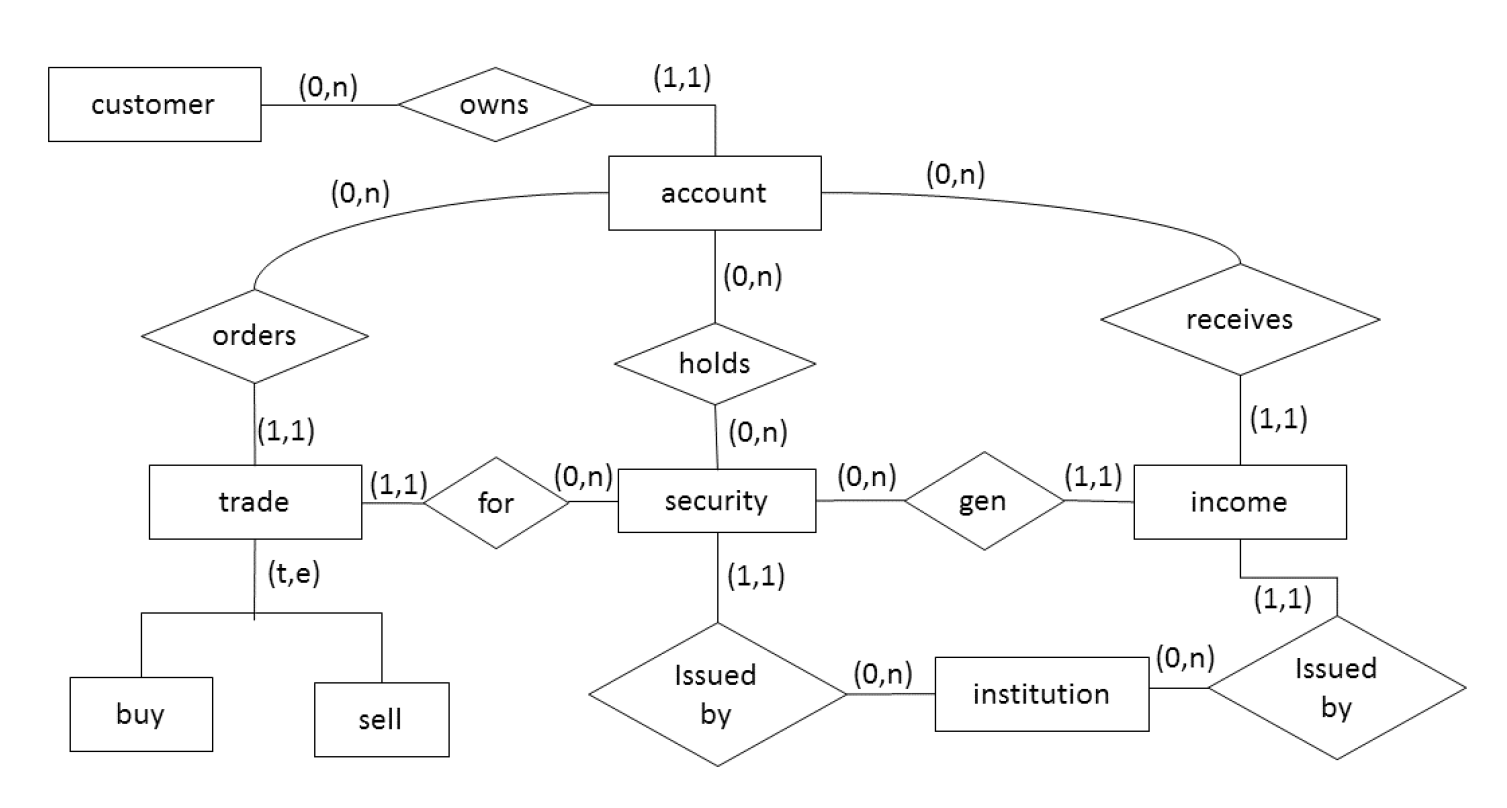
\includegraphics[width=15cm]{unit-11/figures/ER-model.png}
%   \caption*{The structure of a packet frame.}
\end{figure}
\end{center}
The main entities are:
\begin{itemize}
  \item \texttt{customer}
  \item \texttt{account}
  \item \texttt{security}
  \item \texttt{trade}
  \item \texttt{income}
\end{itemize}

Optionally, we may also treat an institution as an entity. We may define subclass entities for buying and selling trade transactions.

\bigskip

% \noindent \textbf{TikZ ER Diagram:}
% \begin{center}
% \begin{tikzpicture}[node distance=2cm, every node/.style={draw, font=\small}]
%   \node (customer) {Customer};
%   \node[below of=customer] (account) {Account};
%   \node[below of=account] (trade) {Trade};
%   \node[right of=account, xshift=4cm] (security) {Security};
%   \node[below of=security] (income) {Income};
%   \node[above right=1.5cm and 2cm of security] (institution) {Institution};

%   \draw (customer) -- node[left]{1..n} (account);
%   \draw (account) -- node[below left]{1..n} (trade);
%   \draw (account) -- node[below]{0..n} (security);
%   \draw (trade) -- node[below]{1} (security);
%   \draw (account) -- node[below right]{0..n} (income);
%   \draw (income) -- node[right]{1} (security);
%   \draw (security) -- node[right]{1} (institution);
% \end{tikzpicture}
% \end{center}



Comments: Almost all the relationships use (1,1) for unique and (0,n) for ``many". For example, an account is owned by a single customer. So it participates in the ``owns" relationship exactly once. A customer may own many accounts.

It is acceptable to use (1,n) for the ``many" multiplicity, but not ideal because it can cause problems in abnormal situations. For example, if the only account of a customer is to be deleted, then the customer would end up with fewer than 1 account.

The many-to-many relationship between account and security is crucial.

It is possible to treat income as a relationship, between account, security and institution. It results in the same tables as this design. \texttt{trade} can also be treated as a relationship (perhaps as two separate relations for ``buys" and ``sells").

It is okay to omit the institution entirely as an entity, because nothing is needed about it other than its name.

\textbf{(b) Logical Design with Relational Schemas} \\

\begin{verbatim}
customer(custid, lastname, firstname, address, email)
account(accid, custid, cash)
security(ISIN, symbol, name, institution)
institution(name, address)
acc_security(accid, security)
trade(tradeid, accid, security, buy_or_sell, qty, date, time, price, commission)
income(accid, security, date, type, amount)
\end{verbatim}

Comments:

We need a table for every entity, except institution, which can possibly be treated as an attribute.

Only one relationship, \texttt{holds}, needs a table, here written as \texttt{acc\_security}.

All other relationships can be absorbed into entities.
\begin{itemize}
  \item \texttt{owns} absorbed into \texttt{account}.
  \item \texttt{orders} and \texttt{for} absorbed into \texttt{trade}.
  \item \texttt{issued by} absorbed into \texttt{security}.
  \item \texttt{issued by} for \texttt{income} also absorbed into \texttt{income}.
\end{itemize}

Note that we do not store the quantity of security held in the account, because it would be redundant: it can be calculated by looking through the trades for that security. If a student stores the quantity as an attribute, make a comment on it, but do not deduct points.

We keep a single table for \texttt{trade}, subsuming both the subclasses into it. It is also possible to have two separate tables for purchases and sales, or three tables: \texttt{trade}, \texttt{purchases} and \texttt{sales}.

\textbf{(c) SQL \texttt{CREATE TABLE} Statements} \\

\begin{verbatim}
create table customer(
  custid INTEGER not null unique primary key,
  lastname VARCHAR(15) not null,
  firstname VARCHAR(15) not null,
  address VARCHAR(100) not null,
  phone DECIMAL(15) not null,
  email VARCHAR(100) not null
);

create table account(
  accid INTEGER not null unique primary key,
  custid INTEGER not null REFERENCES customer(custid),
  cash DECIMAL(10,2) not null
);

create table security(
  ISIN VARCHAR(10) not null unique,
  symbol VARCHAR(4) not null unique,
  name VARCHAR(100) not null,
  institution VARCHAR(20) not null REFERENCES institution(name)
);

create table institution(
  name VARCHAR(20) not null unique PRIMARY KEY,
  address VARCHAR(100) not null
);

create table acc_security(
  accid INTEGER not null REFERENCES account(accid) ON DELETE CASCADE,
  security VARCHAR(10) not null REFERENCES security(ISIN),
  primary key (accid, ISIN)
);

create table trade(
  tradeid INTEGER not null PRIMARY KEY GENERATED ALWAYS BY IDENTITY,
  accid INTEGER not null REFERENCES account(accid) ON DELETE CASCADE,
  security VARCHAR(10) not null REFERENCES security(ISIN),
  buy_or_sell SMALLINT,
  qty INTEGER not null,
  date DATE not null,
  time TIME not null,
  price DECIMAL(10,2) not null,
  commission DECIMAL(4,2) not null
);

create table income(
  accid INTEGER not null REFERENCES account(accid) ON DELETE CASCADE,
  security VARCHAR(10) not null REFERENCES security(ISIN),
  date DATE not null,
  type CHAR not null,
  amount DECIMAL(10,2) not null
);
\end{verbatim}

Most of the \texttt{ON DELETE} constraints are not written in the solution above, which means that the default of \texttt{ON DELETE NO ACTION} would be used.

It is possible to say \texttt{ON DELETE SET NULL} for the references to clients and workers, but then the \texttt{not null} constraint should be deleted.

\texttt{ON DELETE CASCADE} is used for references to accounts, since when an account is deleted, all its transactions have no further relevance.

\textbf{Note:} When an account is to be closed, all the securities held in it would need to be liquidated and the final cash balance would need to be paid out. Only after all this is done should the account be deleted, at which time its trades etc. can be deleted automatically.

On the other hand, we are prohibiting a customer from being deleted when their account still exists. The account should be closed and deleted before the customer can be deleted.

